% !TEX encoding = UTF-8 Unicode
\chapter{Planning}

\begin{figure}[h]
    \begin{center}
        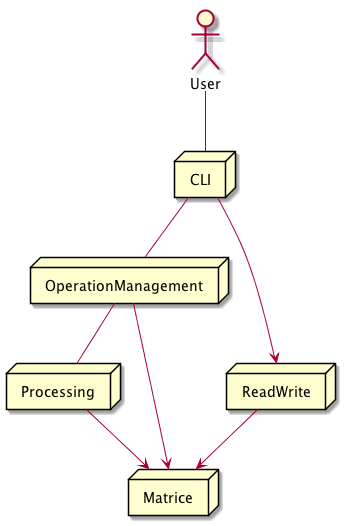
\includegraphics[scale=0.40]{./ressources/graph/deployment.png}
    \end{center}
    \caption{Deployment diagram}
    \label{Solution - Deployment diagram}
\end{figure}
\bigskip

\Section{Backlogs}
\begin{enumerate}
    \item Project structure - 1/2d

    \item Command line interface - 1/2d
    \begin{enumerate}
        \item user interface
        \item user entries processing
        \item unit tests
    \end{enumerate}

    \item Matrice - 1d
    \begin{enumerate}
        \item Matrice data structure
        \item formatting algorithm
        \ unit tests - matrice access, simple research
    \end{enumerate}

    \item Operations management 3h

    \item Search features 1d
    \begin{enumerate}
        \item search management
        \item search algorithm
        \item units test
    \end{enumerate}

    \item FileProcessor 1d
    \begin{enumerate}
        \item read/write
        \item uncryption
        \item file processing
        \item unit tests
    \end{enumerate}

\end{enumerate}

\Section{Sprints}
\subSection{Sprint 1}
Sprint 1 should take 1.5 day. This time will be used to review further the application organisation.
It will contain the initialisation of the application code structure, and a simple command line interface.

    1 - Project structure
    2 - Command line interface

\subSection{Sprint 2}
Sprint 2 should take around 2,5 days. It implies the implementation of reading and processing method for
the plain text file representing our 2 dimensional matrix of integers.
This sprint implies review of algorithm to encrypt/unencrypt file.
And a data structure validating criteria necessary to an optimal research in matrice.

    6 - File processor
    3 - Matrice

\subSection{Sprint 3}
Sprint 3 should take around 2,3 days.
It contain the implementation operation management and 3 types research algorithms responding to requested features.
It implies the validation of research criteria (speed optimisation and valid result), and full workflow testing.

    4 - Operations management
    5 - Search features
    6 - Workflow validation
